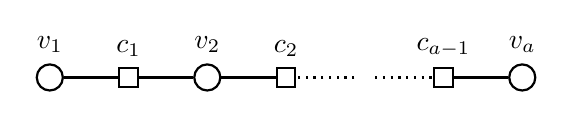
\begin{tikzpicture}[thick,scale=0.5]
\node[circle,draw=black,label={$v_1$}] (v1) at (-4,0){};
\node[circle,draw=black,label={$v_2$}] (v2) at (0,0){};
\node[circle,draw=black,label={$v_a$}] (v3) at (8,0){};

\node[shape=rectangle,draw=black,label={$c_1$}] (c1) at (-2,0){};
\node[shape=rectangle,draw=black,label={$c_2$}] (c2) at (2,0){};
\node[shape=rectangle,draw=black,label={$c_{a-1}$}] (c3) at (6,0){};

\node[shape=rectangle,draw=white,label={}] (p) at (4,0){};

\path [-,thick] (v1) edge node[left] {} (c1); 
\path [-,thick] (v2) edge node[left] {} (c1);
\path [-,thick] (v2) edge node[left] {} (c2);
\path [-,dotted] (p) edge node[left] {} (c2);
\path [-,dotted] (p) edge node[left] {} (c3);
\path [-,thick] (v3) edge node[left] {} (c3);
\end{tikzpicture}